\documentclass[10pt,conference]{IEEEtran}
\usepackage[utf8]{inputenc}
\usepackage[T1]{fontenc}
\usepackage[rm={oldstyle=false}]{cfr-lm}
\usepackage[australian,american]{babel}

\usepackage[backend=biber,style=ieee,bibencoding=utf8,sorting=none,doi=false,isbn=false,url=false,date=short]{biblatex}
\usepackage{csquotes}
\usepackage[caption=false]{subfig}
\usepackage[nolist]{acronym}
\usepackage[binary-units,per-mode=symbol]{siunitx}
\usepackage{float}
\usepackage{todonotes}
\usepackage{pgfplots}
\usepackage{booktabs}
\usepackage{multirow}
\usepackage{lipsum}
\usepackage[hidelinks]{hyperref}

%% Added by Hugues
\usepackage{amsmath, amssymb}

%% Environment for comments: Set the boolean to false to produce a comment-free version.
\newboolean{showcomments}
\setboolean{showcomments}{true}
\ifthenelse{\boolean{showcomments}}
{ \newcommand{\mynote}[3]{
    \fbox{\bfseries\sffamily\scriptsize#1}
    {\small$\blacktriangleright$\textsf{\emph{\color{#3}{#2}}}$\blacktriangleleft$}}}
{ \newcommand{\mynote}[3]{}}
% One command per author:
\newcommand{\hm}[1]{\mynote{Hugues}{#1}{orange}}
\newcommand{\vs}[1]{\mynote{Valerio}{#1}{red}}

\newif\ifjmcs
% Change false to true to have the JMCS cover page
\jmcsfalse

\pgfplotsset{
    compat=1.12,
    tick label style={font=\small},
    label style={font=\small},
    legend style={font=\small},
}

\usepgfplotslibrary{external, dateplot, groupplots, units}
\tikzexternalize
\tikzsetexternalprefix{generated-figures/}

% Columns balancing, enable before final pass
%\renewbibmacro{finentry}{%
%    \iffieldequalstr{entrykey}{fta-paper}%<- key after which you want the break
%    {\finentry\newpage}
%    {\finentry}}

% Constants
\def\mytitle{Master Thesis}
\def\thesistitle{Thesis title}
\def\thesissubtitle{Thesis subtitle}
\def\myauthor{Sébastien Vaucher, Hugues Mercier, Valerio Schiavoni}

\author{\IEEEauthorblockN{\myauthor}
    \IEEEauthorblockA{University of Neuchâtel, Switzerland\\
        \href{mailto:first.last@unine.ch}{first.last@unine.ch}}
}
\title{\mytitle}

\addbibresource{references.bib}
\renewcommand*{\bibfont}{\small}

\hypersetup{
	pdftitle=\mytitle,
	pdfauthor=\myauthor
}

% \noautocite{*}

\begin{document}

\ifjmcs
\begin{titlepage}
    \begin{otherlanguage}{australian}
        \begin{center}
            \begin{figure}[t]
                \center{\includegraphics[scale=0.2]{logos/MSc_quer.png}}
                \vspace{0.4in}
            \end{figure}

            {\bfseries\Huge \thesistitle \par
                \Large \vspace{0.1in} \thesissubtitle \par}

            \vspace{0.3in}
            \LARGE{\textbf{Master Thesis} \\}
            \vspace{0.4in}

            {\Large \myauthor}

            \vspace{0.3in}
            {\Large Université de Neuchâtel \par}
            \vfill
            {\Large \today \par}

            \vspace{0.9in}

            % === Logos ==============================================
            \begin{figure}[htp]
                \centering
                \subfloat{\includegraphics[scale=0.60]{logos/UNI_Bern.pdf}}\hfill
                \subfloat{\includegraphics[scale=0.54]{logos/UNI_Neuchatel.pdf}}\hfill
                \subfloat{\includegraphics[scale=0.81]{logos/UNI_Fribourg.pdf}}
            \end{figure}
            % === // Logos ===========================================

        \end{center}
    \end{otherlanguage}
\end{titlepage}

\pagebreak
\fi

\maketitle

\begin{abstract}
\hm{Should ``storage'' be in the title?} We present ErasureBench, a framework to test and compare erasure coding implementations for distributed storage under realistic conditions. \hm{Expand description.} As a first example, we use ErasureBench to compare three coding implementations: a partition of the data source in ten pieces without error-correction, a (14,10) Reed-Solomon code, and a (10,6,5) locally repairable code. \hm{Conclude}
\end{abstract}


\chapter{Introduction}

The business-model of many major consumer-facing Cloud providers like Dropbox consists in storing huge volumes of data.
Customers expect a high level of reliability, but rarely envisage paying top dollar for that.
It is uncommon to here\vs{hear?} about losses of data affecting users of these kind of services.\vs{you can cite statistics, reports or journal that provide numbers about this.}
To offer that kind of guarantees towards their customers, Cloud providers need to implement techniques providing redundancy, while keeping costs under control.
Unfortunately, hardware components always eventually fail\vs{add a reference. It's easy to find those for hard-disks for instance}.
Laws of probability\vs{which one?} tell us that the likelihood of having one component in a system fail increases with the size of that system.
Therefore, this implies that fault-tolerance needs to be intrinsically built into the design of large-scale systems.

The long-established way of providing redundancy is \vs{replication}: to duplicate functionality across components that are unlikely to fail simultaneously.
As far as data storage is concerned, this means storing multiple carbon copies in geographically distinct locations.
The cost of storage is multiplied by the amount of redundancy wanted.
From an engineering point-of-view, the complexity of that kind of setup is manageable\vs{not clear: what do you mean by manageable?}.

A second\vs{instead of second, i'd say: alternative} solution to providing data redundancy can be constructed using mathematics.
This concept is called erasure-coding and consists in transforming original data in a longer, fault-tolerant form.
Erasure-coding can provide the same level of reliability as replication\vs{add a reference here, it's not straightforward}, but with much less storage overhead.
Computational cost is the main drawback of erasure coding.
Every write to an erasure-coded system requires computing parity blocks.
When reading data back from a replicated data storage system, unavailable blocks can be retrieved by requesting them from another redundant copy.
Reading degraded erasure-coded data implies retrieving a larger amount of blocks than would be needed to read intact data.
Also, some computations need to be performed on the blocks retrieved in order to recreate the unavailable block.
In some cases, like when Facebook tried to apply Reed-Solomon to its data \autocite{XorbasVLDB}, these overheads may prove to be unmanageable in practice.

The newer generation of erasure codes focuses on reducing the amount of data needed for repairing blocks.
That family of codes are named \acp{lrc}\vs{the acroniym is LRC, not LRCs}.
The authors of \autocite{XorbasVLDB} check their claims by using a full-fledged cluster from Facebook.
Not every researcher can have access to that kind of hardware\vs{which hardware?}.
\vs{in the next paragraph, you should explain a bit more extensively what are your contributions: design, implementation and evaluation  of a platform to test different EC techniques as fault-tolerance support for cloud-based storages, a Fuse-enabled system, scalability tests for Redis, use of real-world traces, etc. }
Therefore, we decided to develop a system that can be used to benchmark different erasure code implementations using a reasonable amount of hardware.
Furthermore, our system is not a simulator, so it provides results that should be closer to what would be observed in the real world.

\todo[inline]{This report is structured... Firstly... Secondly...}


\section{Related work}

\subsection{XORing Elephants: Novel Erasure Codes for Big Data}

The article \autocite{XorbasVLDB} presents a new family of erasure codes called \acp{lrc}.
These codes enable local repair of faulty data.
With traditional erasure codes like Reed-Solomon, the cumulative size of the blocks needed to repair a file has to be bigger or equal than the original size of the file.
With \ac{lrc}, a failure affecting a small number of blocks can be repaired using a smaller number of clean blocks.
The authors implemented their algorithm in Hadoop HDFS and deployed a test to Facebook clusters.
They measured that the repair process of \ac{lrc} uses half the disk and network bandwidth compared to Reed-Solomon, at the expense of \SI{14}{\percent} more storage overhead.

\subsection{A Performance Evaluation of Erasure Coding Libraries for Cloud-Based Data Stores}

The authors evaluate the performances of different erasure coding libraries \autocite{Burihabwa2016}.
In order to do the job, they developed a system that is similar to the one presented in this paper.
Their system is mainly geared towards the measurement of read/write throughput and data storage overhead of each erasure coding algorithm.
The algorithms that they tested are implemented in low-level languages.
The interface that their system exposes is a REST API exposed through HTTP.

\vs{to include \url{https://www.cs.utexas.edu/~lorenzo/papers/Silberstein14Lazy.pdf} }

\vs{to include and explain the differences: \url{https://www.usenix.org/legacy/event/fast08/wips_posters/luo-wip.pdf} cite this: 
@phdthesis{Luo:2011:HDI:2338412,
 author = {Luo, Jianqiang},
 advisor = {Xu, Lihao},
 title = {Hyfs: Design and Implementation of a Reliable File System},
 year = {2011},
 isbn = {978-1-124-86527-0},
 note = {AAI3469996},
 publisher = {Wayne State University},
 address = {Detroit, MI, USA},
}
}

\begin{figure}
    \centering
    % TikZ figure showing the relations between all components of the erasure codes tester

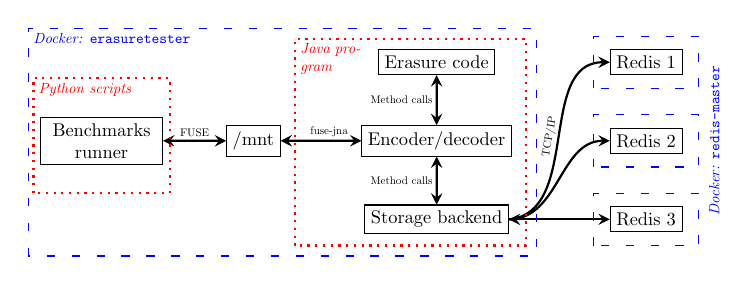
\begin{tikzpicture}[transform shape,scale=0.665]
\node[draw, text width=2.1cm, text centered] (bench) at (2.6, 1.5) {Benchmarks runner};
\node[draw] (dir) at (5.5, 1.5) {/mnt};
\node[draw] (fed) at (9, 1.5) {Encoder/decoder};
\node[draw] (sb) at (9, 0) {Storage backend};
\node[draw] (ec) at (9, 3) {Erasure code};
\node[draw] (r1) at (13, 3) {Redis 1};
\node[draw] (r2) at (13, 1.5) {Redis 2};
\node[draw] (r3) at (13, 0) {Redis 3};

\draw[<->,thick,>=stealth] (bench) -- (dir) node[midway,above,scale=0.6]{FUSE};
\draw[<->,thick,>=stealth] (dir) -- (fed) node[pos=0.6,above,scale=0.6]{fuse-jna};
\draw[<->,thick,>=stealth] (fed) -- (ec)
node[pos=0.5,left,scale=0.6]{Method calls};
\draw[<->,thick,>=stealth] (fed) -- (sb)
node[pos=0.5,left,scale=0.6]{Method calls};
\draw[->,thick,>=stealth] (sb.east) to[out=5,in=180] node[sloped,midway,scale=0.6,above]{TCP/IP} (r1.west);
\draw[->,thick,>=stealth,out=0,in=180] (sb.east) to[out=0,in=180] (r2.west);
\draw[<->,thick,>=stealth] (sb.east) -- (r3.west);

\draw[loosely dashed,blue] (1.2,-0.7) rectangle (10.9,3.65);
\draw[loosely dashed,blue] (12,2.5) rectangle (14,3.5);
\draw[loosely dashed,blue] (12,1) rectangle (14,2);
\draw[loosely dashed,blue] (12,-0.5) rectangle (14,0.5);
\draw[dotted,red,thick] (6.3,-0.5) rectangle (10.7,3.45);
\draw[dotted,red,thick] (1.3,0.5) rectangle (3.9,2.7);

\draw (6.3,3.45) node[below right,red,scale=0.8, text width=1.5cm] {\textit{Java program}};
\draw (1.3,2.7) node[below right,red,scale=0.8] {\textit{Python scripts}};
\draw (1.2,3.65) node[below right,blue,scale=0.8] {\textit{Docker:} \texttt{erasuretester}};
\draw (14.3,1.5) node[blue,scale=0.8,rotate=90] {\textit{Docker:} \texttt{redis-master}};
\end{tikzpicture}

    \caption{Graphical representation of the components of the system}
    \label{fig:architecture}
\end{figure}

\section{ErasureBench code tester}

The ErasureBench code tester is a program written in Java that exposes a filesystem to the user.
It saves files in a key-value store after processing them with an erasure coding algorithm.
Each of the three components (filesystem interface, key-value store, erasure code) can be replaced to test different implementations against each other. While the Java program can be used standalone, it is designed to run in a Docker container shared with associated Python scripts.

\subsection{Software architecture}
\label{subsec:architecture}

The system architecture is summarized in \autoref{fig:architecture}. The Java program exposes a filesystem by using the \ac{fuse} interface. When the user runs the program, the filesystem is mounted under a directory of his choice. The tester intercepts system calls by making use of the \textit{fuse-jna} \autocite{fuse-jna} Java library. Read and write calls are passed through to the encoder/decoder layer.

The encoder/decoder handles the task of correctly chunking file contents.
Its role includes the handling of aligning read and write operations to the correct boundaries.
Once file contents are chunked in data blocks of the correct size, they are passed to the erasure coding algorithm, which adds redundancy blocks.
Data blocks and parity blocks are then passed to the storage backend, which will handle the storage of blocks in a key-value store.

\subsubsection{Available implementations}

As stated in \autoref{subsec:architecture}, each component of our tester can have several implementations.
The frontend has one available implementation: a \ac{fuse} filesystem interface backed by \textit{fuse-jna} \autocite{fuse-jna}.
The encoder/decoder layer is not modular because it is sufficient to have one correct way of handling that operation.
There are three erasure coding algorithms bundled with the program.
They come from \autocite{XorbasVLDB}, and were adapted to free them from dependencies on any \textit{Hadoop} component.
A fourth algorithm is provided, in the name of the \textit{Null} encoder.
As its name suggests, its \textit{modus operandi} consists in simply forwarding data blocks without any added redundancy.
Failing to read a data block while using the \textit{Null} encoder signifies the loss of the stripe associated with it.

Our program is compatible with the \textit{Redis} distributed key-value store through the \textit{Jedis} library.
For testing purposes, a storage backend using an in-memory hash map is also available.

\subsubsection{Blocks storage}

\begin{figure}[H]
    \centering
    % TikZ figure showing how blocks are splitted and encoded

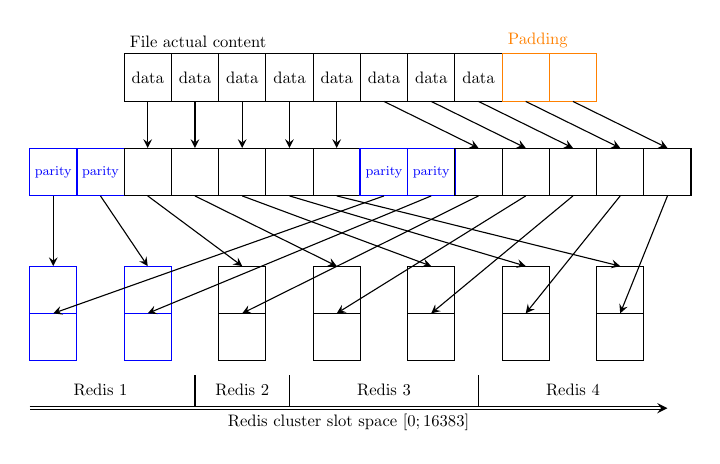
\begin{tikzpicture}[transform shape,scale=0.6]
\draw (1.5,0.5) node[above right] {File actual content};
\node (d1) at (2,0) [draw,minimum width=1cm,minimum height=1cm] {data};
\node (d2) at (3,0) [draw,minimum width=1cm,minimum height=1cm] {data};
\node (d3) at (4,0) [draw,minimum width=1cm,minimum height=1cm] {data};
\node (d4) at (5,0) [draw,minimum width=1cm,minimum height=1cm] {data};
\node (d5) at (6,0) [draw,minimum width=1cm,minimum height=1cm] {data};
\node (d6) at (7,0) [draw,minimum width=1cm,minimum height=1cm] {data};
\node (d7) at (8,0) [draw,minimum width=1cm,minimum height=1cm] {data};
\node (d8) at (9,0) [draw,minimum width=1cm,minimum height=1cm] {data};
\draw (9.5,0.5) node[above right,orange] {Padding};
\node (d9) at (10,0) [orange,draw,minimum width=1cm,minimum height=1cm] {};
\node (d10) at (11,0) [orange,draw,minimum width=1cm,minimum height=1cm] {};

\node (p1) at (0,-2) [draw,minimum width=1cm,minimum height=1cm,blue] {\footnotesize parity};
\node (p2) at (1,-2) [draw,minimum width=1cm,minimum height=1cm,blue] {\footnotesize parity};
\node (p3) at (2,-2) [draw,minimum width=1cm,minimum height=1cm] {};
\node (p4) at (3,-2) [draw,minimum width=1cm,minimum height=1cm] {};
\node (p5) at (4,-2) [draw,minimum width=1cm,minimum height=1cm] {};
\node (p6) at (5,-2) [draw,minimum width=1cm,minimum height=1cm] {};
\node (p7) at (6,-2) [draw,minimum width=1cm,minimum height=1cm] {};
\node (p8) at (7,-2) [draw,minimum width=1cm,minimum height=1cm,blue] {\footnotesize parity};
\node (p9) at (8,-2) [draw,minimum width=1cm,minimum height=1cm,blue] {\footnotesize parity};
\node (p10) at (9,-2) [draw,minimum width=1cm,minimum height=1cm] {};
\node (p11) at (10,-2) [draw,minimum width=1cm,minimum height=1cm] {};
\node (p12) at (11,-2) [draw,minimum width=1cm,minimum height=1cm] {};
\node (p13) at (12,-2) [draw,minimum width=1cm,minimum height=1cm] {};
\node (p14) at (13,-2) [draw,minimum width=1cm,minimum height=1cm] {};

\draw[->,>=stealth] (d1.south) to (p3.north);
\draw[->,>=stealth] (d2.south) to (p4.north);
\draw[->,>=stealth] (d3.south) to (p5.north);
\draw[->,>=stealth] (d4.south) to (p6.north);
\draw[->,>=stealth] (d5.south) to (p7.north);
\draw[->,>=stealth] (d6.south) to (p10.north);
\draw[->,>=stealth] (d7.south) to (p11.north);
\draw[->,>=stealth] (d8.south) to (p12.north);
\draw[->,>=stealth] (d9.south) to (p13.north);
\draw[->,>=stealth] (d10.south) to (p14.north);

\node (r1) at (0,-4.5) [blue,draw,minimum width=1cm,minimum height=1cm] {};
\node (r2) at (2,-4.5) [blue,draw,minimum width=1cm,minimum height=1cm] {};
\node (r3) at (4,-4.5) [draw,minimum width=1cm,minimum height=1cm] {};
\node (r4) at (6,-4.5) [draw,minimum width=1cm,minimum height=1cm] {};
\node (r5) at (8,-4.5) [draw,minimum width=1cm,minimum height=1cm] {};
\node (r6) at (10,-4.5) [draw,minimum width=1cm,minimum height=1cm] {};
\node (r7) at (12,-4.5) [draw,minimum width=1cm,minimum height=1cm] {};

\node (r8) at (0,-5.5) [blue,draw,minimum width=1cm,minimum height=1cm] {};
\node (r9) at (2,-5.5) [blue,draw,minimum width=1cm,minimum height=1cm] {};
\node (r10) at (4,-5.5) [draw,minimum width=1cm,minimum height=1cm] {};
\node (r11) at (6,-5.5) [draw,minimum width=1cm,minimum height=1cm] {};
\node (r12) at (8,-5.5) [draw,minimum width=1cm,minimum height=1cm] {};
\node (r13) at (10,-5.5) [draw,minimum width=1cm,minimum height=1cm] {};
\node (r14) at (12,-5.5) [draw,minimum width=1cm,minimum height=1cm] {};


\draw[->,>=stealth] (p1.south) to (r1.north);
\draw[->,>=stealth] (p2.south) to (r2.north);
\draw[->,>=stealth] (p3.south) to (r3.north);
\draw[->,>=stealth] (p4.south) to (r4.north);
\draw[->,>=stealth] (p5.south) to (r5.north);
\draw[->,>=stealth] (p6.south) to (r6.north);
\draw[->,>=stealth] (p7.south) to (r7.north);
\draw[->,>=stealth] (p8.south) to (r8.north);
\draw[->,>=stealth] (p9.south) to (r9.north);
\draw[->,>=stealth] (p10.south) to (r10.north);
\draw[->,>=stealth] (p11.south) to (r11.north);
\draw[->,>=stealth] (p12.south) to (r12.north);
\draw[->,>=stealth] (p13.south) to (r13.north);
\draw[->,>=stealth] (p14.south) to (r14.north);

\node (redis1) at (1,-6.6) {Redis 1};
\draw (3,-6.3) to (3,-6.95);
\node (redis1) at (4,-6.6) {Redis 2};
\draw (5,-6.3) to (5,-6.95);
\node (redis1) at (7,-6.6) {Redis 3};
\draw (9,-6.3) to (9,-6.95);
\node (redis1) at (11,-6.6) {Redis 4};
\draw[->,>=stealth,double] (-0.5,-7) to node[midway,below]{Redis cluster slot space $\left[0;16383\right]$} (13,-7);

\end{tikzpicture}

    \caption{Representation of the process of splitting file contents in blocks, applying erasure coding to them, and finally storing them in a Redis cluster.}
    \label{fig:blocks}
\end{figure}

The storage backend is designed to operate on 1 byte blocks.
Storing each block individually in the key-value store is a very slow operation.
The metadata accompanying each request to the key-value store server is much bigger than the data itself, leading to unworkable overheads.
We therefore decided to add an intermediate layer between the encoder/decoder and the storage backend.

This layer is transparent to the encoder/decoder which still deals with single 1 byte blocks.
Thanks to this new layer, multiple write operations on the key-value store are aggregated.
Instead of storing one block per key, each key stores an aggregation of multiple blocks.
The guarantees offered by the erasure coding process are still kept because one aggregation only stores blocks that belong to the same stripe position.
This additional component provides a considerable speed-up comprised between $100\times$ and $1000\times$.
The way files are split in blocks, erasure coded and then aggregated to be stored on multiple Redis servers is shown in \autoref{fig:blocks}.

A \ac{lru} cache optimizes the retrieval of multiple individuals blocks.
This way, when reading a file sequentially, each aggregation of blocks is only retrieved once from the key-value store.

\subsubsection{Metadata storage}

When storing file contents in the storage cluster, we need to keep track where each block gets stored.
The strategy we adopted is to assign a 32 bits key to each block.
From each key, we can infer two related identifiers: a Redis key and an offset.
The Redis key points to an aggregation of blocks stored into the Redis cluster.
We then use the offset to precisely locate the block we want within the aggregation.

We store all metadata in memory.
Each file consists in a list of identifiers.
We also store the size of the file once decoded, so we can discard padding blocks.
Naturally, the space overhead of our solution is important, so our system is not able to store a large amount of data.

\subsection{Surrounding components}

Running the tester requires multiple independent services.
They need to be launched simultaneously and need to be bootstrapped to work together.
On top of these services, we want to perform measurements on the performance of different erasure codes.
The solution we adopted is the containerization of each service.
The tester along with supporting Python scripts are bundled together in a Docker image.
When an experimenter wants to start the benchmarks with, say, a 20 nodes Redis cluster as storage backend, he only needs to specify the desired setup in a configuration file.
The supporting Python scripts will configure the Redis cluster and then run the benchmarks and collect the results.
We use the \textit{redis-trib.rb} script to initialize the Redis cluster.
We also used it to scale the cluster, but it was too slow if there were more than a dozen nodes.
We therefore implemented the same logic in our own Python scripts, so we can scale the cluster much faster.

Thanks to the use of Docker Swarm, the setup to run the benchmarks on a local machine or on a cluster of machines is similar.
The system can use any reasonable number of Redis servers.
We provide shell scripts that automate the complete pipeline, from the compilation of sources to the execution of benchmarks on a remote Docker swarm cluster.

\subsection{Faults simulation}

The goal of erasure codes is to provide fault tolerance.
In order to test this aspect, we want to introduce faults in the system.
To that end, we added the possibility to specify a failure trace when running an experiment.
There are two types of failures traces that our program accepts: synthetic traces and real traces.
A synthetic trace is simply a list of system sizes.
When a benchmark completes a loop, the storage cluster is resized using the next value in the list.

Real failure traces take the form of SQLite databases.
The are filled by monitoring individual nodes of a real-life distributed system, and recording failure events in said database.
Our tester can then replay these traces to replicate a real-world failure pattern.
A storage cluster of the same size as the original system will be created.
New nodes will be instantiated and old nodes killed at the same rate as recorded in the trace.
For convenience, the user can specify a limited timeframe of the trace to use.
It is also possible to accelerate or decelerate the trace.


\begin{figure*}[t]
    \centering
    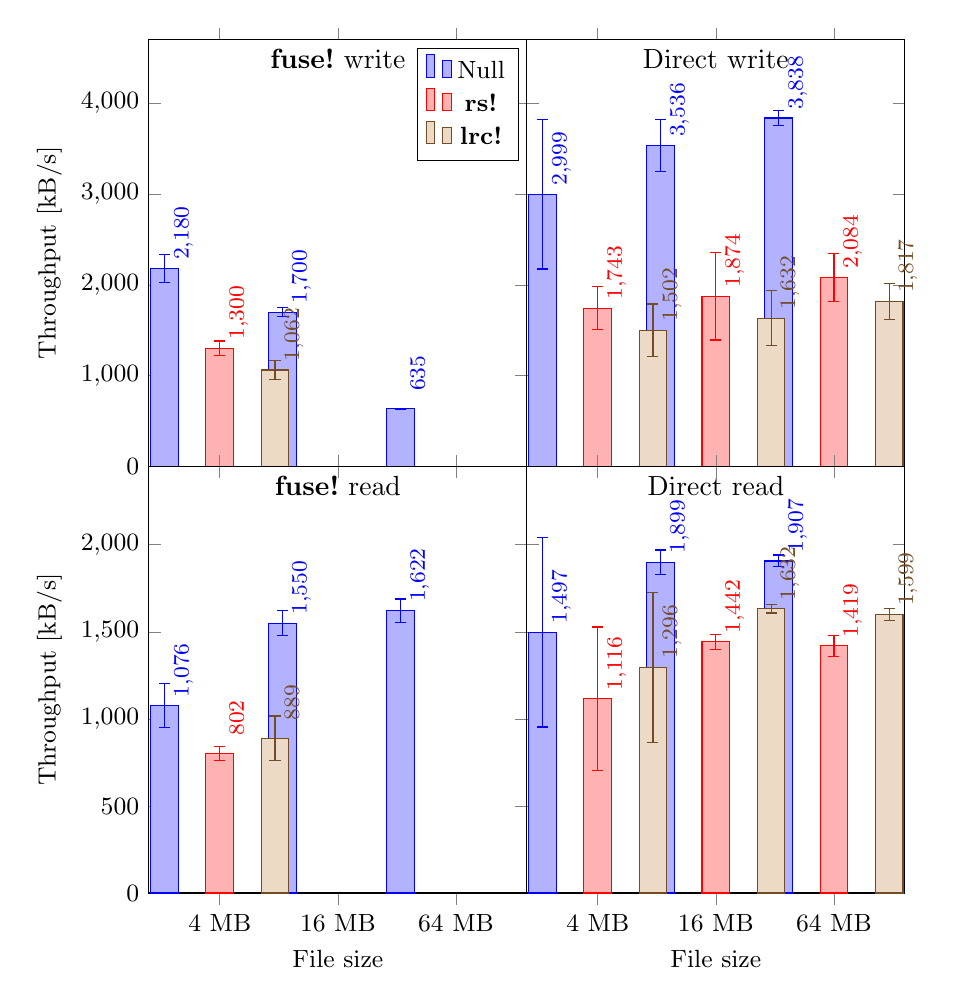
\begin{tikzpicture}
\usetikzlibrary{plotmarks}
\pgfplotsset{width=\linewidth, height=7cm}
\begin{groupplot}[
    group style={
        group size=2 by 2,
        vertical sep=0pt,
        horizontal sep=0pt,
        xlabels at=edge bottom,
        ylabels at=edge left,
        xticklabels at=edge bottom,
        yticklabels at=edge left
    },
    ymin=0,
%    ytick={0,500,1000,...,2500},
    width=\linewidth / 1.9,
    enlarge x limits=0.3,
    ybar=3.5mm,
    nodes near coords,
    every node near coord/.append style={
        rotate=90,
        anchor=north,
        font=\footnotesize,
        xshift=4.5mm
    },
    xtick=data,
    xlabel=File size,
    ylabel={Throughput $\left[\text{kB/s}\right]$},
    symbolic x coords={4 MB, 16 MB, 64 MB}
]
\nextgroupplot[ymax=4700]
% Write with FUSE
\addplot+[error bars/.cd,y dir=both, y explicit] coordinates {
    % Write
    (4 MB, 2180) +- (0, 154.92)
    (16 MB, 1700) +- (0, 47.14)
    (64 MB, 635) +- (0, 4.42)
};
\addplot+[error bars/.cd,y dir=both, y explicit] coordinates {
    % Write
    (4 MB, 1300) +- (0, 81.65)
};
\addplot+[error bars/.cd,y dir=both, y explicit] coordinates {
    % Write
    (4 MB, 1062) +- (0, 100.49)
};

\legend{Null, \acs{rs}, \acs{lrc}}

% Write direct
\nextgroupplot[ymax=4700]
% Null
\addplot+[error bars/.cd,y dir=both, y explicit] coordinates {
    % Write
    (4 MB, 2999) +- (0, 824.6)
    (16 MB, 3536) +- (0, 289.1)
    (64 MB, 3838) +- (0, 81.1)
};
% RS
\addplot+[error bars/.cd,y dir=both, y explicit] coordinates {
    % Write
    (4 MB, 1743) +- (0, 235.5)
    (16 MB, 1874) +- (0, 481.6)
    (64 MB, 2084) +- (0, 264.5)
};
% LRC
\addplot+[error bars/.cd,y dir=both, y explicit] coordinates {
    % Write
    (4 MB, 1502) +- (0, 287.6)
    (16 MB, 1632) +- (0, 301.6)
    (64 MB, 1817) +- (0, 197.3)
};

\nextgroupplot[ymax=2450]
% Read with FUSE
\addplot+[error bars/.cd,y dir=both, y explicit] coordinates {
    % Read
    (4 MB, 1076) +- (0, 127.74)
    (16 MB, 1550) +- (0, 70.71)
    (64 MB, 1622) +- (0, 66.67)
};
\addplot+[error bars/.cd,y dir=both, y explicit] coordinates {
    % Read
    (4 MB, 802) +- (0, 41.76)
};
\addplot+[error bars/.cd,y dir=both, y explicit] coordinates {
    % Read
    (4 MB, 889) +- (0, 127.61)
};

% Read direct
\nextgroupplot[ymax=2450]
% Null
\addplot+[error bars/.cd,y dir=both, y explicit] coordinates {
    % Read
    (4 MB, 1497) +- (0, 543.6)
    (16 MB, 1899) +- (0, 71.2)
    (64 MB, 1907) +- (0, 34.1)
};
% RS
\addplot+[error bars/.cd,y dir=both, y explicit] coordinates {
    % Read
    (4 MB, 1116) +- (0, 411.9)
    (16 MB, 1442) +- (0, 44.8)
    (64 MB, 1419) +- (0, 58.7)
};
% LRC
\addplot+[error bars/.cd,y dir=both, y explicit] coordinates {
    % Read
    (4 MB, 1296) +- (0, 432.4)
    (16 MB, 1632) +- (0, 24.0)
    (64 MB, 1599) +- (0, 33.1)
};
\end{groupplot}

\node[anchor=north] at (group c1r1.north) {\acs{fuse} write};
\node[anchor=north] at (group c1r2.north) {\acs{fuse} read};
\node[anchor=north] at (group c2r1.north) {Direct write};
\node[anchor=north] at (group c2r2.north) {Direct read};
\end{tikzpicture}

    \caption{Throughput of different erasure coding algorithms with different file sizes on a storage cluster of 100 nodes. Half confidence interval.\vs{increase space between plots, move title outside the plot, remove border around legend, make it less tall}}
    \label{fig:throughput-plot}
\end{figure*}

\section{Evaluation}
\label{sec:evaluation}

This section presents the evaluation of our \SYS prototype. 
First, we describe the evaluation settings in \autoref{sec:eval:settings}.
Then we evaluate several characteristics of the system: network throughput, encoding/decoding, request latency and scalability.
We conclude our evaluation by assessing its fault tolerance features by mean of synthetic and real-world traces.
\vs{add refs to specific sections the text is stable}.

\subsection{Evaluation Settings}
\label{sec:eval:settings}

We deploy our experiments over a cluster of machines interconnected by a \SI{1}{\giga\bit\per\second} switched network.
Each physical host features an octocore Intel Xeon CPU and \SI{8}{\giga\byte} of RAM.
We deploy \acp{vm} on top of the hosts.
The KVM hypervisor, which controls the execution of the \acp{vm}, is configured to expose the physical CPU to the guest \ac{vm} and Docker containers by mean of the \texttt{host-passthrough} option.
The \acp{vm} leverage the \texttt{virtio} module for better I/O performance.
We deploy Docker (v1.11) containers on each VM without any memory restrictions.
We use Docker Compose (v1.7.1) and Docker Swarm (v1.11.2) to orchestrate the deployment of the containers in our cluster.

\subsection{Workloads}
\label{sec:eval:workloads}
%we evaluate the various aspects or our tester by comparing two data coding algorithms against unprocessed data.
%The two algorithms under test are \acf{rs} and \acf{lrc}.
In order to evaluate the performance of \SYS, we selected the source files of two well-known open-source projects: the Apache \texttt{httpd}\footnote{\url{https://archive.apache.org/dist/httpd/httpd-2.4.18.tar.bz2}} server (v2.4.18) and GNU \texttt{bc}\footnote{\url{https://ftp.gnu.org/gnu/bc/bc-1.06.tar.gz}} (v1.06). 
We chose them because they differ in the total number of files and storage requirements, as can be seen in \autoref{fig:overhead-table}.
Moreover, we created a synthetic archive containing 1000 files, each consisting of 10 random bytes (\SI{10}{\byte} in the remainder).
We store and read files contained in these archives from the \SYS's \ac{fuse} filesystem. 
\vs{STOPPED HERE}

\begin{figure}
    \centering
    \begin{tikzpicture}
\usetikzlibrary{plotmarks}
\pgfplotsset{every axis plot post/.append style={
        solid,
        thick,
        mark size=1pt
    }
}
\begin{axis}[
    xlabel=Dead nodes,
    ylabel=Available files,
    cycle list name=exotic
]
\addplot table[x=bench-apache-Null-x, y=bench-apache-Null-y] {plots/checksum-100nodes.dat};
\addlegendentry{httpd-2.4.18 / Null}
\addplot table[x=bench-10bytes-Null-x, y=bench-10bytes-Null-y] {plots/checksum-100nodes.dat};
\addlegendentry{10 bytes / Null}

\addplot table[x=bench-apache-SimpleRegenerating-x, y=bench-apache-SimpleRegenerating-y] {plots/checksum-100nodes.dat};
\addlegendentry{httpd-2.4.18 / \acs{lrc}}
\addplot table[x=bench-10bytes-SimpleRegenerating-x, y=bench-10bytes-SimpleRegenerating-y] {plots/checksum-100nodes.dat};
\addlegendentry{10 bytes / \acs{lrc}}

\addplot table[x=bench-apache-ReedSolomon-x, y=bench-apache-ReedSolomon-y] {plots/checksum-100nodes.dat};
\addlegendentry{httpd-2.4.18 / \acs{rs}}
\addplot table[x=bench-10bytes-ReedSolomon-x, y=bench-10bytes-ReedSolomon-y] {plots/checksum-100nodes.dat};
\addlegendentry{10 bytes / \acs{rs}}
\end{axis}
\end{tikzpicture}

    \caption{Fault tolerance of: no erasure coding (Null), \acl{lrc} $\left(10,6,5\right)$ and \acl{rs} $\left(10,4\right)$. Data written on 100 nodes, and then read after killing each node.\vs{remove border around legend, reduce lenght of the horiz bar for each element}}
    \label{fig:checksum-plot}
\end{figure}

\subsection{Fault-tolerance}
\label{subsec:fault-tolerance}

One of the most important, or perhaps the most important characteristic of an erasure coding algorithm is its tolerance to faults.
A good code should ensure that data stays completely available when a small fraction of servers goes down.
We quantified the fault tolerance of \acf{rs}, \acf{lrc} and no erasure coding.
We instantiated a storage cluster of 100 nodes, and extracted the contents of an archive in it.
We used 2 different archives: \SI{10}{\byte}, which is an ideal scenario and httpd, which is our real-world scenario.
After the files were extracted, we checked the integrity of each file contained in the storage cluster.
We then killed storage nodes one after the other, and checked the files integrity before each step.

\autoref{fig:checksum-plot} shows the availability ratio of individual files with regard to the ratio of dead nodes.
It shows that \ac{rs} provides better fault-tolerance than \ac{lrc}.
It also demonstrates that the larger files contained in httpd are more prone to failures, as a single damaged stripe within a file will corrupt the entire file.

\subsection{Read/write performance and overhead of \acs{fuse}}
\label{subsec:rw-perf}

The plot in \autoref{fig:throughput-plot} shows the user-facing throughput of the system.
We write three files of different sizes and containing random data to the filesystem, and then read them.
To measure the \textit{\ac{fuse}} case, read and write operations are performed against the mountpoint exposed by the tester.
The \textit{Direct} case bypasses the \ac{fuse} layer, and directly calls Java methods.

For all cases except \textit{\ac{fuse} write}, we can see that larger file sizes yield better results.
Performance when writing increasingly bigger files using \ac{fuse} decreases because some buffers have to be resized as the file grows.
Larger writes lead to more resizing operations.

\ac{rs} is faster in writing than \ac{lrc}, notably because it requires less blocks to be written to the system,
On read operations, \ac{lrc} is inherently faster as it requires the same number of blocks as \ac{rs}.

The decrease in performance caused by \ac{fuse} ranges between \SI{-19.8}{\percent} and \SI{-41}{\percent} for read operations, and between \SI{-33.6}{\percent} and \SI{-84.9}{\percent} for write operations.

\begin{table*}
    \centering
    \caption{Various metrics measured when storing files in the system.\vs{use same names as those in the plots}}
    \sisetup{table-format=4.0}
\begin{tabular}{
        l
        c
        c
        l
        S[table-format=5.0]
        S[table-format=3.2]
        S[table-format=3.2]
}
\toprule
\multirow{2}{*}{Name} & \multirow{2}{*}{Files} & \multirow{2}{*}{Size} & \multicolumn{1}{c}{Erasure} & {Redis} & {Binary} & {Base64} \\
& & & \multicolumn{1}{c}{code} & {keys} & {blocks} & {blocks} \\

\midrule

% 10 bytes
\multirow{3}{*}{\SI{10}{\byte}} & \multirow{3}{*}{\tablenum{1000}} & \multirow{3}{*}{\tablenum[table-format=2.2]{0.01}} & NC
           & 10000 & 0.12 & 0.16 \\
 & & & RS  & 14000 & 0.17 & 0.22 \\
 & & & LRC & 16000 & 0.19 & 0.26 \\

\addlinespace
% bc-1.06
\multirow{3}{*}{bc} & \multirow{3}{*}{\tablenum{94}} & \multirow{3}{*}{\tablenum[table-format=2.2]{1.02}} & NC
           & 1920 & 4.09 & 5.45 \\
 & & & RS  & 2688 & 5.72 & 7.63 \\
 & & & LRC & 3072 & 6.54 & 8.73 \\

\addlinespace
% httpd-2.4.18
\multirow{3}{*}{httpd} & \multirow{3}{*}{\tablenum{2516}} & \multirow{3}{*}{\tablenum[table-format=2.2]{33.02}} & NC
           & 56850 & 132.68 & 176.99 \\
 & & & RS  & 79590 & 185.75 & 247.79 \\
 & & & LRC & 90960 & 212.29 & 283.18 \\
\bottomrule
\end{tabular}

    \label{fig:overhead-table}
\end{table*}

\subsection{Storage overheads}
\label{subsec:storage-overheads}

\autoref{fig:overhead-table} shows various metrics relative to the storage space used when unpacking 4 different archives into the filesytem exposed by the tester.
The \enquote{10 bytes} archive constitutes a worst case, as each file is stored as a single stripe in the system.
In that case, the number of Redis keys is strictly equal to the number of blocks in the system.
Storing a 10 bytes file into our system takes 120 bytes, before base 64 applied.
Each byte is encoded as a 32 bits integer by the erasure codes.
Additionally, each aggregation of blocks needs two 32 bits integers to store its decoded size.
This explains the overhead of $12\times$.
For real archives, the overhead asymptotically approaches $4\times$, as the two 32 bits integers are only needed once per aggregation.

The overheads cited above reason upon the binary size.
As Redis can only store strings, we have to apply base 64 encoding to the blocks, adding \SI{33}{\percent} storage overhead.

The overhead due to erasure coding is always governed by the number of parity blocks added.

\begin{figure}
    \centering
    \begin{tikzpicture}
\usetikzlibrary{plotmarks}
\pgfplotsset{width=\linewidth, height=7cm}
\begin{axis}[
    x unit=s,
    xlabel=Duration,
    ylabel=CDF,
    cycle list name=exotic,
    cycle list shift=1,
    legend pos=south east,
]
\addplot+ table[x index=0, y index=5] shell {./gencdf.rb -f plots/latency.csv -c 1};
\addplot+ table[x index=0, y index=5] shell {./gencdf.rb -f plots/latency.csv -c 2};
\addplot+ table[x index=0, y index=5] shell {./gencdf.rb -f plots/latency.csv -c 3};
\addplot+ table[x index=0, y index=5] shell {./gencdf.rb -f plots/latency.csv -c 4};
\legend{20 nodes, 40 nodes, 60 nodes, 80 nodes}
\end{axis}
\end{tikzpicture}

    \caption{Cumulative distribution of the latency observed when writing a \SI{16}{\mebi\byte} file to a storage cluster without erasure coding.\vs{use same form factor of Fig 4, remove border around legend, reduce lenght of the horiz bar for each element }}
    \label{fig:latency-plot}
\end{figure}

\subsection{Cluster size impact on latency}
\label{subsec:latency}

In order to test the impact of the cluster size on performances, we measured the time needed to write \SI{16}{\mebi\byte} to storage clusters of various sizes.
The results are shown as a \ac{cdf} in \autoref{fig:latency-plot}.
We can see that the growth of the cluster size has an impact on performance, although it is limited.

\begin{figure*}
    \centering
    \begin{tikzpicture}
\usetikzlibrary{plotmarks}
\pgfplotsset{every axis plot post/.append style={
        solid,
        mark size=1.7pt
    },
    height=6.5cm,
    width=\linewidth,
}
\begin{axis}[
    xlabel={Elapsed time $\left[\si{\second}\right]$},
    ylabel={Network throughput $\left[\si{\mega\byte\per\second}\right]$},
    ymax=34000000,
    cycle list name=exotic,
    cycle list shift=1,
    legend style={
        anchor=north,
        at={(0.5,0.97)},
    },
    legend cell align=left,
    legend columns=2,
    scaled y ticks=base 10:-6,
    ytick scale label code/.code={},
]
\addplot table[x=write-100nodes-ReedSolomon-x, y=write-100nodes-ReedSolomon-y] {plots/throughput.dat};
\addplot table[x=write-100nodes-SimpleRegenerating-x, y=write-100nodes-SimpleRegenerating-y] {plots/throughput.dat};
\addplot table[x=read-normal-100nodes-ReedSolomon-x, y=read-normal-100nodes-ReedSolomon-y] {plots/throughput.dat};
\addplot table[x=read-normal-100nodes-SimpleRegenerating-x, y=read-normal-100nodes-SimpleRegenerating-y] {plots/throughput.dat};
\addplot table[x=read-degraded-100nodes-ReedSolomon-x, y=read-degraded-100nodes-ReedSolomon-y] {plots/throughput.dat};
\addplot table[x=read-degraded-100nodes-SimpleRegenerating-x, y=read-degraded-100nodes-SimpleRegenerating-y] {plots/throughput.dat};

\legend{RS write, LRC write, RS read, LRC read, RS deg. read, LRC deg. read}
\end{axis}
\end{tikzpicture}

    \caption{Network throughput between the encoder and 100 Redis storage servers when the httpd archive is written and then read. 5 nodes are brutally killed before measuring a degraded read.}
    \label{fig:traffic-plot}
\end{figure*}

\subsection{Network traffic to/from storage nodes}
\label{subsec:network-traffic}

We evaluated the network capacity used by \ac{rs} and \ac{lrc}.
We extracted the \textit{httpd} archive into the system while monitoring network traffic between the encoder and all Redis storage nodes.
We then did the reverse operation, once with all storage nodes intact, and once after killing \SI{5}{\percent} of the nodes.

The results are displayed in \autoref{fig:traffic-plot}.
They show that \ac{lrc} needs more time to complete at roughly the same speed as \ac{rs}, due to 2 more blocks per stripe.
For read operations, \ac{lrc} is equivalent to \ac{rs} when the cluster is intact.
The notable characteristic of \ac{lrc} is its increased block locality compared to \ac{rs}.
We can clearly observe that it effectively lowers the network usage as far as degraded reads are concerned.

\begin{figure}
    \centering
    \begin{tikzpicture}
\usetikzlibrary{plotmarks}
\pgfplotsset{every axis plot post/.append style={
        solid,
        thick,
        mark size=1pt
    }
}
\begin{axis}[
    xlabel=Dead nodes,
    ylabel=Available files,
    cycle list name=exotic
]
%\addplot table[x=timestamp, y=size] {plots/websites-size.dat};
\end{axis}
\end{tikzpicture}

    \caption{Top plot: graphical representation of the number of nodes available at a given time as recorded in the trace file. Bottom plots: network traffic incurred by writing \textit{httpd} to the storage cluster, moving blocks between servers when scaling up, and repairing blocks when nodes die.}
    \label{fig:trace-plot}
\end{figure}

\subsection{Impact of real faults on network usage}
\label{subsec:fault-trace}

One of the unique features of our erasure codes tester is the possibility to replicate recorded failure patterns.
We used this feature to evaluate the impact on network throughput when faults happen.
We replicated a \SI{7}{\hour} subset of the fault trace recorded by the authors of \autocite{websites02}.
We initialized our cluster with 117 machines, and extracted the \textit{httpd} archive in it.
During the whole experiment, we tracked the network traffic occurring at the storage nodes.
Then, when a new node joined the system, we migrated some blocks towards it.
When an existing node departed, we scrubbed the blocks stored in the system and repaired incomplete stripes.

In \autoref{fig:trace-plot}, the uppermost plot shows the size of the storage cluster.
An increase indicates a node joining the system while a decrease marks a failure.
The two plots in the lower part of \autoref{fig:trace-plot} show the network throughput that was observed when erasure coding the data using \ac{rs} versus \ac{lrc}.


\section{Conclusion}
\label{sec:conclusion}
The evaluation of erasure coding libraries in a realistic context is a difficult matter.
The usual approach explored in literature is to rely on simulations.
This however negatively impact the outcome and the lessons learned that practitioners and researchers can exploit. 
In this paper we design, implement and evaluate ErasureBench, a modular framework to overcome these limitations.
ErasureBench offers a familiar file-system interface, it allows to plug different erasure-coding libraries, to inject real-world failure traces and to deploy locally or on a cluster without major modifications to the code.
We test the validity of our prototype by evaluating the cost of two different erasure coding algorithms, based respectively on Reed-Solomon and on Locally Repairable Codes.
Our evaluation confirm well-known theoretical results on the efficiency of \ac{lrc} codes in a large-scale setting.  



\begin{acronym}
\acro{lrc}[LRC]{Locally Repairable Code}
\end{acronym}


\printbibliography

\end{document}
